\section{Arquitetura e Componentes do Wiki.js}

O projeto, que nos foi apresentado, consiste no planeio e operacionalização da instalação de uma plataforma \textbf{Wiki.js}, tal como toda a manutenção necessária ao seu bom funcionamento. Para esse efeito, começamos por desenvolver a arquitetura que servirá como base de todo o trabalho.

A aplicação \textbf{Wiki.js} encontra-se dividida entre \textit{frontend}, que apresentará a interface ao \textit{web client}, e \textit{backend} e utilizará uma base de dados para o armazenamento de dados:

\begin{figure}[h]
    \centering
    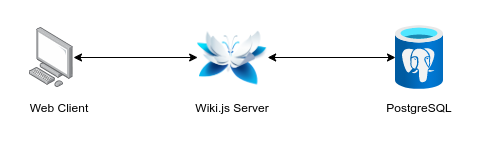
\includegraphics[width=\linewidth]{img/wiki_basic_arch.png}
    \caption{Diagrama da arquitetura do sistema}
    \label{fig_1}
\end{figure}

\subsection{Servidor Wiki.js}

\textbf{Wiki.js} é uma aplicação \textit{open source}, escrita em JavaScript e que corre em Node.js, oferecendo a funcionalidade de gerar páginas wiki completamente customizáveis e modulares.

Para além de ser uma aplicação web extremamente rápida e ter um design simplista e elegante, possui um vasto conjunto de ferramentas \textit{dev friendly} e oferece suporte para a base de dados \textbf{PostgreSQL} \cite{wiki-article}.

Numa primeira intalação (simplificada), esta plataforma, ficará instalada num servidor individual (servidor aplicacional). Aquando da comunicação pelos utilizadores, \textit{web clients}, terá de fornecer o \textit{frontend} ou camada de apresentação. Para além disso, o \textit{backend} irá comunicar com o servidor de base de dados, onde será armazenada toda a informação.

\subsection{Servidor PostgreSQL}

Tal como referido previamente, o nosso servidor aplicacional comunica (escrita e leitura de dados) diretamente com uma base de dados \textbf{PostgreSQL}, que estará instalada no seu próprio servidor.

Decidimos recorrer a este sistema de gestão de base de dados por vários motivos. Primeiramente, a própria documentação da plataforma \textbf{Wiki.js} recomenda o seu uso, \cite{wiki-requirements}. Depois, é o sistema mais popular do mercado e ganhou a sua extensa reputação devido à sua arquitetura, confiabilidade, integridade de dados, vasta gama de \textit{features} e dedicação à comunidade \textit{open source}. Além disso, está presente em todos os maiores sistemas operativos \cite{postgres-about}. Por fim, achamos que o facto de já estarmos acostumados à sua utilização, se mostraria uma mais valia na realização deste projeto.

\pagebreak